\documentclass[journal,onecolumn]{IEEEtran}




% *** MISC UTILITY PACKAGES ***
%
%\usepackage{ifpdf}
% Heiko Oberdiek's ifpdf.sty is very useful if you need conditional
% compilation based on whether the output is pdf or dvi.
% usage:
% \ifpdf
%   % pdf code
% \else
%   % dvi code
% \fi
% The latest version of ifpdf.sty can be obtained from:
% http://www.ctan.org/pkg/ifpdf
% Also, note that IEEEtran.cls V1.7 and later provides a builtin
% \ifCLASSINFOpdf conditional that works the same way.
% When switching from latex to pdflatex and vice-versa, the compiler may
% have to be run twice to clear warning/error messages.






% *** CITATION PACKAGES ***
%
%\usepackage{cite}
% cite.sty was written by Donald Arseneau
% V1.6 and later of IEEEtran pre-defines the format of the cite.sty package
% \cite{} output to follow that of the IEEE. Loading the cite package will
% result in citation numbers being automatically sorted and properly
% "compressed/ranged". e.g., [1], [9], [2], [7], [5], [6] without using
% cite.sty will become [1], [2], [5]--[7], [9] using cite.sty. cite.sty's
% \cite will automatically add leading space, if needed. Use cite.sty's
% noadjust option (cite.sty V3.8 and later) if you want to turn this off
% such as if a citation ever needs to be enclosed in parenthesis.
% cite.sty is already installed on most LaTeX systems. Be sure and use
% version 5.0 (2009-03-20) and later if using hyperref.sty.
% The latest version can be obtained at:
% http://www.ctan.org/pkg/cite
% The documentation is contained in the cite.sty file itself.






% *** GRAPHICS RELATED PACKAGES ***
%
\ifCLASSINFOpdf
\usepackage[pdftex]{graphicx}
  % declare the path(s) where your graphic files are
  % \graphicspath{{../pdf/}{../jpeg/}}
  % and their extensions so you won't have to specify these with
  % every instance of \includegraphics
  % \DeclareGraphicsExtensions{.pdf,.jpeg,.png}
\else
  % or other class option (dvipsone, dvipdf, if not using dvips). graphicx
  % will default to the driver specified in the system graphics.cfg if no
  % driver is specified.
  % \usepackage[dvips]{graphicx}
  % declare the path(s) where your graphic files are
  % \graphicspath{{../eps/}}
  % and their extensions so you won't have to specify these with
  % every instance of \includegraphics
  % \DeclareGraphicsExtensions{.eps}
\fi
% graphicx was written by David Carlisle and Sebastian Rahtz. It is
% required if you want graphics, photos, etc. graphicx.sty is already
% installed on most LaTeX systems. The latest version and documentation
% can be obtained at: 
% http://www.ctan.org/pkg/graphicx
% Another good source of documentation is "Using Imported Graphics in
% LaTeX2e" by Keith Reckdahl which can be found at:
% http://www.ctan.org/pkg/epslatex
%
% latex, and pdflatex in dvi mode, support graphics in encapsulated
% postscript (.eps) format. pdflatex in pdf mode supports graphics
% in .pdf, .jpeg, .png and .mps (metapost) formats. Users should ensure
% that all non-photo figures use a vector format (.eps, .pdf, .mps) and
% not a bitmapped formats (.jpeg, .png). The IEEE frowns on bitmapped formats
% which can result in "jaggedy"/blurry rendering of lines and letters as
% well as large increases in file sizes.
%
% You can find documentation about the pdfTeX application at:
% http://www.tug.org/applications/pdftex





% *** MATH PACKAGES ***
%
%\usepackage{amsmath}
% A popular package from the American Mathematical Society that provides
% many useful and powerful commands for dealing with mathematics.
%
% Note that the amsmath package sets \interdisplaylinepenalty to 10000
% thus preventing page breaks from occurring within multiline equations. Use:
%\interdisplaylinepenalty=2500
% after loading amsmath to restore such page breaks as IEEEtran.cls normally
% does. amsmath.sty is already installed on most LaTeX systems. The latest
% version and documentation can be obtained at:
% http://www.ctan.org/pkg/amsmath





% *** SPECIALIZED LIST PACKAGES ***
%
%\usepackage{algorithmic}
% algorithmic.sty was written by Peter Williams and Rogerio Brito.
% This package provides an algorithmic environment fo describing algorithms.
% You can use the algorithmic environment in-text or within a figure
% environment to provide for a floating algorithm. Do NOT use the algorithm
% floating environment provided by algorithm.sty (by the same authors) or
% algorithm2e.sty (by Christophe Fiorio) as the IEEE does not use dedicated
% algorithm float types and packages that provide these will not provide
% correct IEEE style captions. The latest version and documentation of
% algorithmic.sty can be obtained at:
% http://www.ctan.org/pkg/algorithms
% Also of interest may be the (relatively newer and more customizable)
% algorithmicx.sty package by Szasz Janos:
% http://www.ctan.org/pkg/algorithmicx




% *** ALIGNMENT PACKAGES ***
%
%\usepackage{array}
% Frank Mittelbach's and David Carlisle's array.sty patches and improves
% the standard LaTeX2e array and tabular environments to provide better
% appearance and additional user controls. As the default LaTeX2e table
% generation code is lacking to the point of almost being broken with
% respect to the quality of the end results, all users are strongly
% advised to use an enhanced (at the very least that provided by array.sty)
% set of table tools. array.sty is already installed on most systems. The
% latest version and documentation can be obtained at:
% http://www.ctan.org/pkg/array


% IEEEtran contains the IEEEeqnarray family of commands that can be used to
% generate multiline equations as well as matrices, tables, etc., of high
% quality.



\usepackage{amsmath} % special symbols
\usepackage{amssymb} % more special symbols
\usepackage{epsfig} % needed for including figures
\usepackage{lipsum} % generate placeholder text
\usepackage[hyphens]{url} % line break URLs
\usepackage[usenames,dvipsnames,svgnames,table]{xcolor} % custom color definition
\usepackage[figure]{algorithm2e} % advanced written algorithm handling
\usepackage{graphicx} % advanced graphic manipulation handling
\usepackage{epstopdf} % converts vector graphics (eps) to pdf for embedding
\usepackage{longtable} % allows tables to break across multiple pages
\usepackage{makeidx} % create an index
\usepackage{framed}
\usepackage{placeins}
\usepackage{cite}


% *** SUBFIGURE PACKAGES ***
%\ifCLASSOPTIONcompsoc
%  \usepackage[caption=false,font=normalsize,labelfont=sf,textfont=sf]{subfig}
%\else
%  \usepackage[caption=false,font=footnotesize]{subfig}
%\fi
% subfig.sty, written by Steven Douglas Cochran, is the modern replacement
% for subfigure.sty, the latter of which is no longer maintained and is
% incompatible with some LaTeX packages including fixltx2e. However,
% subfig.sty requires and automatically loads Axel Sommerfeldt's caption.sty
% which will override IEEEtran.cls' handling of captions and this will result
% in non-IEEE style figure/table captions. To prevent this problem, be sure
% and invoke subfig.sty's "caption=false" package option (available since
% subfig.sty version 1.3, 2005/06/28) as this is will preserve IEEEtran.cls
% handling of captions.
% Note that the Computer Society format requires a larger sans serif font
% than the serif footnote size font used in traditional IEEE formatting
% and thus the need to invoke different subfig.sty package options depending
% on whether compsoc mode has been enabled.
%
% The latest version and documentation of subfig.sty can be obtained at:
% http://www.ctan.org/pkg/subfig




% *** FLOAT PACKAGES ***
%
%\usepackage{fixltx2e}
% fixltx2e, the successor to the earlier fix2col.sty, was written by
% Frank Mittelbach and David Carlisle. This package corrects a few problems
% in the LaTeX2e kernel, the most notable of which is that in current
% LaTeX2e releases, the ordering of single and double column floats is not
% guaranteed to be preserved. Thus, an unpatched LaTeX2e can allow a
% single column figure to be placed prior to an earlier double column
% figure.
% Be aware that LaTeX2e kernels dated 2015 and later have fixltx2e.sty's
% corrections already built into the system in which case a warning will
% be issued if an attempt is made to load fixltx2e.sty as it is no longer
% needed.
% The latest version and documentation can be found at:
% http://www.ctan.org/pkg/fixltx2e


%\usepackage{stfloats}
% stfloats.sty was written by Sigitas Tolusis. This package gives LaTeX2e
% the ability to do double column floats at the bottom of the page as well
% as the top. (e.g., "\begin{figure*}[!b]" is not normally possible in
% LaTeX2e). It also provides a command:
%\fnbelowfloat
% to enable the placement of footnotes below bottom floats (the standard
% LaTeX2e kernel puts them above bottom floats). This is an invasive package
% which rewrites many portions of the LaTeX2e float routines. It may not work
% with other packages that modify the LaTeX2e float routines. The latest
% version and documentation can be obtained at:
% http://www.ctan.org/pkg/stfloats
% Do not use the stfloats baselinefloat ability as the IEEE does not allow
% \baselineskip to stretch. Authors submitting work to the IEEE should note
% that the IEEE rarely uses double column equations and that authors should try
% to avoid such use. Do not be tempted to use the cuted.sty or midfloat.sty
% packages (also by Sigitas Tolusis) as the IEEE does not format its papers in
% such ways.
% Do not attempt to use stfloats with fixltx2e as they are incompatible.
% Instead, use Morten Hogholm'a dblfloatfix which combines the features
% of both fixltx2e and stfloats:
%
% \usepackage{dblfloatfix}
% The latest version can be found at:
% http://www.ctan.org/pkg/dblfloatfix




% *** PDF, URL AND HYPERLINK PACKAGES ***
%
%\usepackage{url}
% url.sty was written by Donald Arseneau. It provides better support for
% handling and breaking URLs. url.sty is already installed on most LaTeX
% systems. The latest version and documentation can be obtained at:
% http://www.ctan.org/pkg/url
% Basically, \url{my_url_here}.




% *** Do not adjust lengths that control margins, column widths, etc. ***
% *** Do not use packages that alter fonts (such as pslatex).         ***
% There should be no need to do such things with IEEEtran.cls V1.6 and later.
% (Unless specifically asked to do so by the journal or conference you plan
% to submit to, of course. )


% correct bad hyphenation here
\hyphenation{op-tical net-works semi-conduc-tor}


\newcommand{\TODO}[1]{\textcolor{red}{\textbf{TODO: } #1}}



\begin{document}

\title{Identification of Conserved Regions\\ in CRISPR protein family}

% make the title area
\maketitle

\begin{center}
\begin{tabular}{ c c c }
 Christine Baek$^1$ & Qi Chu$^1$ & Yanyu Liang$^1$ \\ 
christib@andrew.cmu.edu & qchu@andrew.cmu.edu & yanyul@andrew.cmu.edu \\     
\end{tabular}\\
\smallskip
\smallskip
$^1$Computational Biology, Carnegie Mellon University
\end{center}

\bigskip

% As a general rule, do not put math, special symbols or citations
% in the abstract
\begin{abstract}
The abstract goes here.
\end{abstract}

% no keywords





\section{Introduction}

\TODO{Christine : brief intro}

\subsection{CRISPR/Cas} 
\TODO{Christine writes about CRISPR bg}
Subsection text here.

\subsection{Past Approaches}
\TODO{Qi : summarize the HMMer approach?}

\subsection{Approaches in This Paper}
\TODO{everyone?}

\subsection{Goal of Paper}
\TODO{Yanyu : short discussion of our goal in this paper}


% An example of a floating figure using the graphicx package.
% Note that \label must occur AFTER (or within) \caption.
% For figures, \caption should occur after the \includegraphics.
% Note that IEEEtran v1.7 and later has special internal code that
% is designed to preserve the operation of \label within \caption
% even when the captionsoff option is in effect. However, because
% of issues like this, it may be the safest practice to put all your
% \label just after \caption rather than within \caption{}.
%
% Reminder: the "draftcls" or "draftclsnofoot", not "draft", class
% option should be used if it is desired that the figures are to be
% displayed while in draft mode.
%
%\begin{figure}[!t]
%\centering
%\includegraphics[width=2.5in]{myfigure}
% where an .eps filename suffix will be assumed under latex, 
% and a .pdf suffix will be assumed for pdflatex; or what has been declared
% via \DeclareGraphicsExtensions.
%\caption{Simulation results for the network.}
%\label{fig_sim}
%\end{figure}

% Note that the IEEE typically puts floats only at the top, even when this
% results in a large percentage of a column being occupied by floats.


% An example of a double column floating figure using two subfigures.
% (The subfig.sty package must be loaded for this to work.)
% The subfigure \label commands are set within each subfloat command,
% and the \label for the overall figure must come after \caption.
% \hfil is used as a separator to get equal spacing.
% Watch out that the combined width of all the subfigures on a 
% line do not exceed the text width or a line break will occur.
%
%\begin{figure*}[!t]
%\centering
%\subfloat[Case I]{\includegraphics[width=2.5in]{box}%
%\label{fig_first_case}}
%\hfil
%\subfloat[Case II]{\includegraphics[width=2.5in]{box}%
%\label{fig_second_case}}
%\caption{Simulation results for the network.}
%\label{fig_sim}
%\end{figure*}
%
% Note that often IEEE papers with subfigures do not employ subfigure
% captions (using the optional argument to \subfloat[]), but instead will
% reference/describe all of them (a), (b), etc., within the main caption.
% Be aware that for subfig.sty to generate the (a), (b), etc., subfigure
% labels, the optional argument to \subfloat must be present. If a
% subcaption is not desired, just leave its contents blank,
% e.g., \subfloat[].


% An example of a floating table. Note that, for IEEE style tables, the
% \caption command should come BEFORE the table and, given that table
% captions serve much like titles, are usually capitalized except for words
% such as a, an, and, as, at, but, by, for, in, nor, of, on, or, the, to
% and up, which are usually not capitalized unless they are the first or
% last word of the caption. Table text will default to \footnotesize as
% the IEEE normally uses this smaller font for tables.
% The \label must come after \caption as always.
%
%\begin{table}[!t]
%% increase table row spacing, adjust to taste
%\renewcommand{\arraystretch}{1.3}
% if using array.sty, it might be a good idea to tweak the value of
% \extrarowheight as needed to properly center the text within the cells
%\caption{An Example of a Table}
%\label{table_example}
%\centering
%% Some packages, such as MDW tools, offer better commands for making tables
%% than the plain LaTeX2e tabular which is used here.
%\begin{tabular}{|c||c|}
%\hline
%One & Two\\
%\hline
%Three & Four\\
%\hline
%\end{tabular}
%\end{table}


% Note that the IEEE does not put floats in the very first column
% - or typically anywhere on the first page for that matter. Also,
% in-text middle ("here") positioning is typically not used, but it
% is allowed and encouraged for Computer Society conferences (but
% not Computer Society journals). Most IEEE journals/conferences use
% top floats exclusively. 
% Note that, LaTeX2e, unlike IEEE journals/conferences, places
% footnotes above bottom floats. This can be corrected via the
% \fnbelowfloat command of the stfloats package.


\section{Methods}

We used 3 differenr approaches .. blahblahblah. All used the same .fa sequence, etc. etc. 
talk about the data itself here, and why we used 3 different methods.
\TODO{Christine : fill in this section, and why protein sequence}

\subsection{Data Retrieval}

\TODO{Qi : talk about source of data}

\subsection{Sequence Alignment using Dynamic Programming}
\subsubsection{Model \& Algorithm Overview}

Semiglobal ailgnment using Needleman-Wunsch~\cite{needlemanwunsch} and Local Alignment using Smith-Waterman Algorithm~\cite{smithwaterman}

\subsubsection{Pros and Cons}
running time is polynomial in terms of number of sequences being aligned. actual global max achieved, for the sequences being aligned. 

\subsubsection{Protocol}
BLOSUM62 used - general good starting point, for varied sequence similarities. 

\subsubsection{Analysis}
Discuss METHOD for analysis, not the actual result/analysis itself. 

\subsection{Gibbs Sampling}
\subsubsection{Model \& Algorithm Overview}
talk about overview of what the method does (method itself, not in detail of how you used it)

\subsubsection{Pros and Cons}
of using the method - what is it capable of, what are the limitations ?

\subsubsection{Protocol}
implementation details - justifications for decisions you made when you ran the experiment, parameters, etc.

\subsubsection{Analysis}
Discuss METHOD for analysis, not the actual result/analysis itself. 


\subsection{Domain-specific profile HMM}
\subsubsection{Model \& Algorithm Overview}
To find out whether a sequence of amino acid belongs some domain, we can build a model of the domain and try to match the sequence of the model. Profile Hidden Markov Model is one of the 
models we can build to figure out whether a sequence contains the domain. The model of profile HMM is shown in Figure \ref{HMM}. 

\begin{figure}[ht]
  \centering
  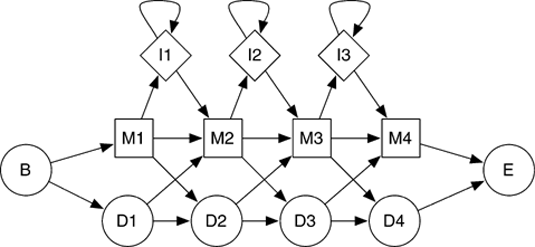
\includegraphics[scale = 0.7]{images/profileHMM}
      \caption{Profile Hidden Markov Model\cite{hmmer}}
      \label{HMM}
\end{figure}


\subsubsection{Pros and Cons}
\begin{itemize}
\item Pros
\begin{enumerate}
\item We can leverage the abundant prior knowledge of Cas9 domain markers by building profile HMM using the alignment of the domains rather than the full sequence.
\item Compared with pair-wise sequence alignment, HMM can find more cases of distantly related sequences.
\item As shown in the figure, HMM can model insertions and deletions.
\end{enumerate}
\item Cons
\begin{enumerate}
\item To leverage the prior knowledge of domain markers, those markers need to be fetched separately from other data source rather than learned by the algorithm.
\item The number of parameters is very large and they need to be optimized.
\end{enumerate}
\end{itemize}

\subsubsection{Protocol}
\begin{enumerate}
\item A set of \textit{Cas9} or \textit{Cas5} sequences and their domain markers are fetched from EMBL-EBI (http://www.ebi.ac.uk).
\item Sequences of each of the shared domains are subtracted from the full \textit{Cas9} or \textit{Cas5} sequences.
\item For each domain, multiple sequences from different \textit{Cas9} or \textit{Cas5} are aligned by Clustal Omega (http://www.clustal.org/).
\item  A profile HMM is built on the multiple sequence alignment for each domain by Hmmer (http://hmmer.org/)\cite{hmmer}.
\item Search for matches using the profile HMM in the sequences of all previously downloaded \textit{Cas} family proteins.
\end{enumerate}

\subsubsection{Analysis}
For method testing, a set of globin sequences given in Hmmer\cite{hmmer} is used. Since there are \textit{Cas9} and \textit{Cas5} in the previously downloaded \textit{Cas} family proteins sequences, they also act as positive control since the method should be able to find the domains in these proteins.\\
For output analysis, HMM is able to give the probability of given sequence emitted from the underlying domain profile HMM.





\section{Results}

Individual results for each 

\TODO{put in appropriate figures, and any analysis for each}


\subsection{Sequence Alignment using Dynamic Programming}

\subsection{Gibbs Sampling}

\subsection{HMM}


\section{Conclusion}


\TODO{we need to do this one together}


% trigger a \newpage just before the given reference
% number - used to balance the columns on the last page
% adjust value as needed - may need to be readjusted if
% the document is modified later
%\IEEEtriggeratref{8}
% The "triggered" command can be changed if desired:
%\IEEEtriggercmd{\enlargethispage{-5in}}

% references section

% can use a bibliography generated by BibTeX as a .bbl file
% BibTeX documentation can be easily obtained at:
% http://mirror.ctan.org/biblio/bibtex/contrib/doc/
% The IEEEtran BibTeX style support page is at:
% http://www.michaelshell.org/tex/ieeetran/bibtex/
%\bibliographystyle{IEEEtran}
% argument is your BibTeX string definitions and bibliography database(s)
%\bibliography{IEEEabrv,../bib/paper}
%
% <OR> manually copy in the resultant .bbl file
% set second argument of \begin to the number of references
% (used to reserve space for the reference number labels box)

\TODO{please include any other resources or papers you referenced}

\begin{thebibliography}{1}

\bibitem{IEEEhowto:kopka}
H.~Kopka and P.~W. Daly, \emph{A Guide to \LaTeX}, 3rd~ed.\hskip 1em plus
  0.5em minus 0.4em\relax Harlow, England: Addison-Wesley, 1999.

\bibitem{cas:makarova}
K. S. ~Makarova, et al., \emph{An updated evolutionary classification of CRISPR-Cas systems}  \hskip 1em plus 0.5em minus 0.4em\relax http://dx.doi.org/10.1038/nrmicro3569, 28 September 2015

\bibitem{needlemanwunsch}
Saul B. Needleman, Christian D. Wunsch, \emph{A general method applicable to the search for similarities in the amino acid sequence of two proteins} \hskip 1em plus 0.5em minus 0.4em\relax http://www.sciencedirect.com/science/article/pii/0022283670900574, 28 March 1970

\bibitem{smithwaterman}
Smith, Temple F. \& Waterman, Michael S., \emph{Identification of Common Molecular Subsequences} \hskip 1em plus 0.5em minus 0.4em\relax Journal of Molecular Biology. 147: 195-197. doi:10.1016/0022-2836(81)90087-5. PMID 7265238., 1981

\bibitem{hmmer}
HMMER 3.1b2 (February 2015); http://hmmer.org/

\end{thebibliography}




\end{document}


